\documentclass{article}

\usepackage[dutch]{babel}
\usepackage[version=3]{mhchem}
\usepackage{hyperref}
\usepackage{pdfpages}
\usepackage{graphicx}
\usepackage{marvosym}
\usepackage{graphicx}
\usepackage{wrapfig}
\usepackage{listings}
\usepackage[gen]{eurosym}
\usepackage{caption}
\usepackage{subcaption}
\usepackage{float}

% Variables for source code colors
\definecolor{dkgreen}{rgb}{0,0.6,0}
\definecolor{gray}{rgb}{0.5,0.5,0.5}
\definecolor{mauve}{rgb}{0.58,0,0.82}

% Makeup for source code display
\lstset{
        language=C++,
        basicstyle={\small\ttfamily},
        numbers=left,
        numberstyle=\small\color{gray},
        numberstyle=\tiny\color{gray},
        keywordstyle=\color{blue},
        commentstyle=\color{dkgreen},
        stringstyle=\color{mauve},
	tabsize=2,
	breaklines=true,
}  
\usepackage{marvosym}
\usepackage{url} 

\begin{document}

\title{Documentatie Pinautomaat}
\author{Bytegroep 10}

\maketitle

\begin{abstract}

De opdracht voor dit project was om een werkende geldautomaat te maken.
In dit verslag zijn onderzoeksanalysen met adviezen terug te vinden.
Wij hebben aan de hand van deze adviezen hierna ontwerpen gemaakt en gerealizeerd.
Wij moeten tijdens de loop van het project letten op vijf onderdelen: \emph{beheren, analyseren, adviseren, ontwerpen en realiseren.}

\end{abstract}

\newpage

\tableofcontents

\newpage

\section{Version control}

Voor dit onderdeel moesten wij kunnen werken met Git en Version control.
Hier is veel onderzoek over gedaan zodat het goed toegepast kan worden dit project.
In figuur \ref{fig: git model} is het model wat wij gebruiken op onze Git pagina, \href{https://github.com/Gewad/Project4Bankalicious}{Project4Bankalicious}.
Ieder groepslid werkt op zijn individuele branch, en als je klaar bent met jouw onderdeel, dan wordt hij in test gemerged.
Als er geen problemen lijken te zijn op de test beslissen wij in een groep of wij test naar de master kunnen schrijven.
Alle documentatie is terug te vinden op Github.

\begin{figure}[!h]
        \centering
        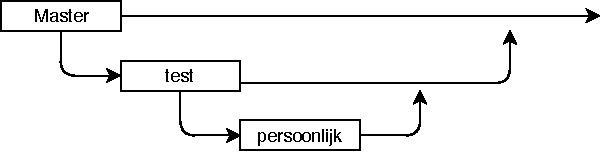
\includegraphics[height=0.7in]{git.pdf}
        \caption{git model}
        \label{fig: git model}
\end{figure}

\section{Samenwerkingscontract}
\label{chap:Samenwerkingscontract}

\paragraph{Financi\"en}

De kosten voor het gezamenlijke deel van de opdracht(en) worden gezamenlijk betaald, iedereen betaald even veel.

\paragraph{Schades}

Als er iets kapot gaat, worden de kosten van het vervangen gedeeld door de groep tenzij er opzettelijk of onverantwoordelijk mee om is gegaan.
In dat geval zullen de kosten voor de persoon die de schade heeft aangericht zijn.

\paragraph{Github afspraken}

\begin{itemize}
\item Niet op de master werken. Je werkt altijd op een eigen kopie van de test branch.
\item Gelieve geen word bestanden te uploaden zonder ook een pdf te uploaden.
\item Commits moeten duidelijk beschrijven wat er is aangepast. Liever een paar woorden teveel dan te weinig.
\item De repo van project 4 is geen zandbak om Git te testen.
\item Directories zijn met kleine letters en underscores, en hebben een duidelijke naam.
\item Alle benamingen en commits moeten in het Nederlands.
\item Branch namen zijn met kleine letters en woorden zijn verbonden met een min teken.
\end{itemize}

\paragraph{Te laat bij afspraken}

Al onze afspraken worden in goed overleg gepland daarom wordt er van groepsleden verwacht
dat ze op tijd zijn bij een afspraak (zowel deadlines als overleg) als een groepslid zonder goede
1
reden meer dan 5 minuten te laat is dan staat daar een consequentie tegen over. Deze
consequentie is of 20 chicken mcnuggets of een taart (let op: cake is geen taart!), als er
meerdere mensen te laat zijn moeten zij allebei iets mee nemen.

\paragraph{Afwezigheid bij afspraken}

Al onze afspraken worden in goed overleg gepland daarom wordt er van groepsleden verwacht
dat ze bij afspraken aanwezig zijn. als een groepslid zonder goede reden afwezig is bij een
overleg staat daar een consequentie tegenover. Deze consequentie is of 40 chicken mcnuggets
of twee taarten. Deze reden zal met de groep besproken moeten worden voordat het een geldige reden is.

\paragraph{Communicatie}

Communiceer goed, dat betekent duidelijk en met respect durf anderen aan te spreken.
Vraag hulp als je hulp nodig hebt.
Geef op tijd aan als je wil stoppen met de studie en draag alle onderdelen van het project tijdig
over aan een ander groepslid.

\paragraph{Rolverdeling}

De rolverdeling staat netjes gedocumenteerd op Github, en ieder teamlid is gediend deze zo
goed mogelijk uit te voeren.
\begin{itemize}
\item Paul H. Organizator
\item Paul W. Verbinder
\item Gerard Expert
\item Merijn Documentatie manager, onderzoeker
\item Aron Tester
\item Boas Kwaliteitsbewaker
\item Floor Designer, expert
\item Mohammed Designer
\end{itemize}

\newpage

\section{Kwaliteitseisen}

%TODO Boas, eisen moeten dit en dat doen.

\subsubsection{Code eisen}
De code eisen:
\begin{itemize}
	\item De bonnentjes printer moet aangeroepen kunnen worden de GUI
	\item De motoren moeten aangestuurd worden door de GUI
	\item De 
\end{itemize}

\subsubsection{Product eisen}
\begin{itemize}
	\item Het product moet 4 verschillende biljetten kunnen uitgeven
	\item Het product moet gebruik maken van motoren om het de biljetten uit te geven
\end{itemize}

\subsubsection{Eindgebruiker eisen}
\subsubsection{Git eisen}

Zie sectie \ref{chap:Samenwerkingscontract} voor de eisen voor onze git pagina.



\section{Analyse \& advies}

\subsection{Dispenser}

Wij hebben onderzoek gedaan naar twee manieren van het uitgeven van biljetten.
Wij hebben vooral onderzoek gedaan bij de tweede jaars.
Optie \'e\'en is om een zuigpomp te gebruiken en de biljetten naar boven te zuigen.
De tweede jaars raden dit af, omdat zij hier zelf geen goede ervaring mee hadden.

Manier twee is om de biljetten uit te werpen met een elektromotor.
De tweede jaars hadden hier goede ervaring mee, dit ding namelijk minder vaak fout bij het uitwerpen.
De elektromotor zal de kaarten uit de dispenser rollen.

Voor het uitgeven van biljetten is het effici\"enter om een elektromotor te gebruiken.
Hier is er meer kans dat het juiste aantal biljetten uit de automaat komen.

\newpage

\subsection{Veiligheid}

\paragraph{Netwerk encryption}

Er is veel onderzoek gedaan naar de beveiliging van het dataverkeer.
Voor netwerken beveiliging heb je een encryptie nodig over het netwerk.
Wij raden aan om hiervoor een bestaand protocol toe te passen.
SSL wordt professioneel toegepast bij bedrijven.
Het kan gewoon gebruikt worden als hij goed toegepast wordt met de meest recente versie.

\paragraph{lokale encryption}

Voor lokale encryption zou je de hele database kunnen encrypten, en decrypten wanneer je data nodig hebt.
Dit kost echter een hoop rekenkracht, en je gegevens zullen op een paar plaatsen onversluiteld zijn.

Een oplossing hiervoor is om gevoelige gegevens te hashen, en vervolgens in de database op te slaan.
Als je bijvoorbeeld wilt controleren of een pincode klopt, zal deze eerst gehasht worden en vervolgens vergeleken met wat er in de database staat.
Een veelgebruikt hashing algoritme voor java en c++, de talen waar wij in programmeren, is bijvoorbeeld md5.
Het is beter om een hashing algoritme te gebruiken wat iets zwaarder is dan md5, omdat je een hash makkelijk terug kunt rekenen.
Een beter veelgebruikt algoritme is bijvoorbeeld SHA1.
Deze adviseren wij te gebruiken.

\hfill

\centerline{\ce{pincode ->[hash] hashed} \ce{pincode} \ce{->[vergelijk] Database met hashes}}

\paragraph{Afgesloten hardware}

Het is heel cruciaal voor de automaat dat buitenstaanders geen toegang hebben tot de logica van de machine en de biljetten.
Om dit te voorkomen is het het handigst om de hardware aan de binnenkant van de automaat te houden.
Wij raden aan om een kast om de functionele onderdelen heel te bouwen, zodat deze niet meer toegankelijk zijn.

\subsection{Biljetten}

Wij hebben eerst aan de tweede jaars gevraagd wat voor soort materiaal wij het best konden gebruiken voor de biljetten.
Zij kwamen met twee opties.
\begin{itemize}
\item Je kan zelf biljetten maken, om ze zo op je model af te stellen.
\item Je kan speelkaarten gebruiken, omdat deze gemaakt zijn om met een dispenser uit te werpen.
\end{itemize}

Wij raden aan voor het gebruik van speelkaarten vanwege de dispencer.
De manier hoe de dispencer gemaakt is zorgt ervoor dat alleen de speelkaarten geschikt zijn voor biljetten.
Wij kunnen direct aan te slag met de dispenser als wij speelkaarten gebruiken, sinds wij deze al hebben.
Er zijn 4 dispencers waarvan elk een bepaald type biljet bevat.
E\'en dispencer bevat biljetten van \euro{5},
een ander van \euro{10},
een ander weer van \euro{20} en \'e\'en van \euro{50}.

\newpage

\subsection{Sensoren}
In een ATM kan er maar een bepaald hoeveelheid van biljetten.
In de ATM moet er bijgehouden worden hoeveel biljetten er zijn uitgegeven.
Om de uitgave ban biljetten te meten gaan wij gebruik maken van sensoren.
Er zullen 4 sensoren gebruikt worden bij elke dispencer.
Elke sensor kan bijhouden hoeveel biljetten van zijn aangewezen dispencer zijn uitgegeven.
In het systeem van de ATM wordt dit geregistreed.

%TODO bouwtekening.
\begin{figure}[H]
	\centering
	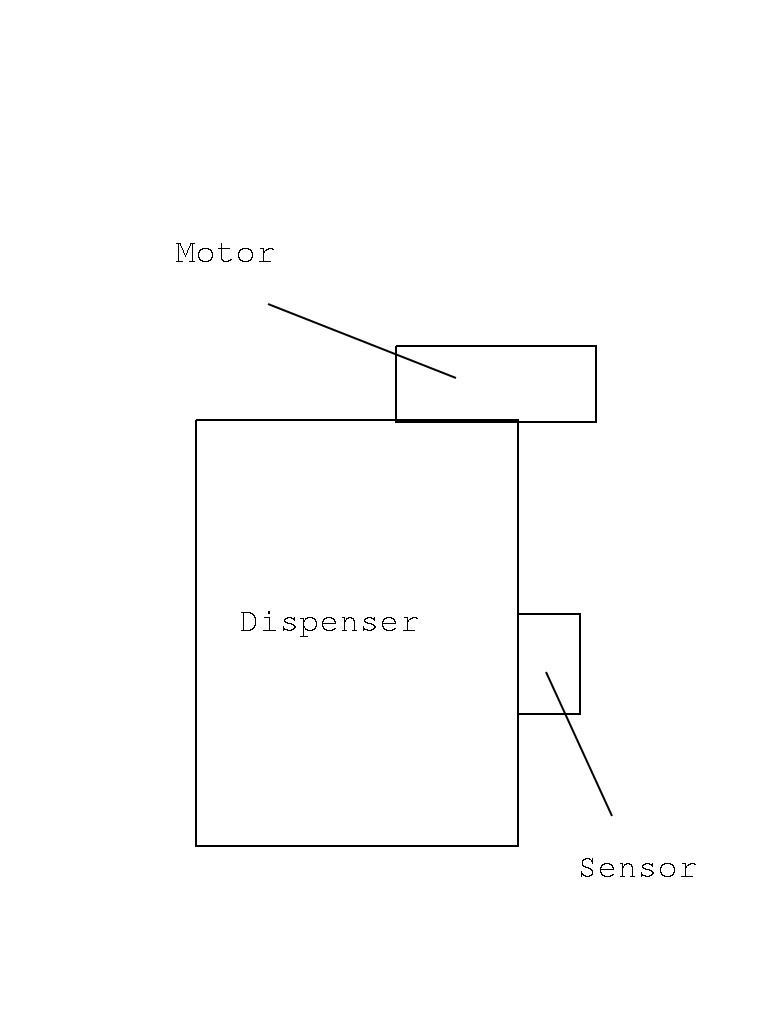
\includegraphics[height=4.5in]{zijkantdispenser.png}
	\caption{Zijaanzicht Dispenser Sensor}
	\label{fig: Zijaanzicht Dispenser Sensor}
\end{figure}

\subsection{Communicatie}

De laptop zal opdrachten sturen naar de Labelprinter en de geld dispenser.
Zie de netwerk diagram in figuur \ref{fig: Netwerk Diagram}

\begin{figure}[H]
        \centering
        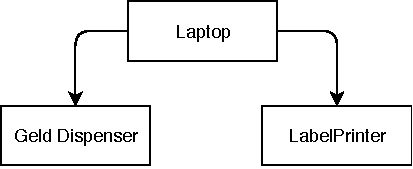
\includegraphics[height=0.9in]{netwerk_diagram.pdf}
        \caption{Netwerk Diagram}
        \label{fig: Netwerk Diagram}
\end{figure}

Hieronder is in pseudocode te zien welke opdrachten de laptop kan versturen naar de verbonden apparaten 
\lstinputlisting{communicatie.pseudo}

Voor de communicatie tussen de klassen in de GUI van de automaat zijn in een diagram weergegeven.
Om deze te bezichten, zie de bijlage.

\newpage
\subsection{Bonnen}

\begin{figure}[H]
        \centering
        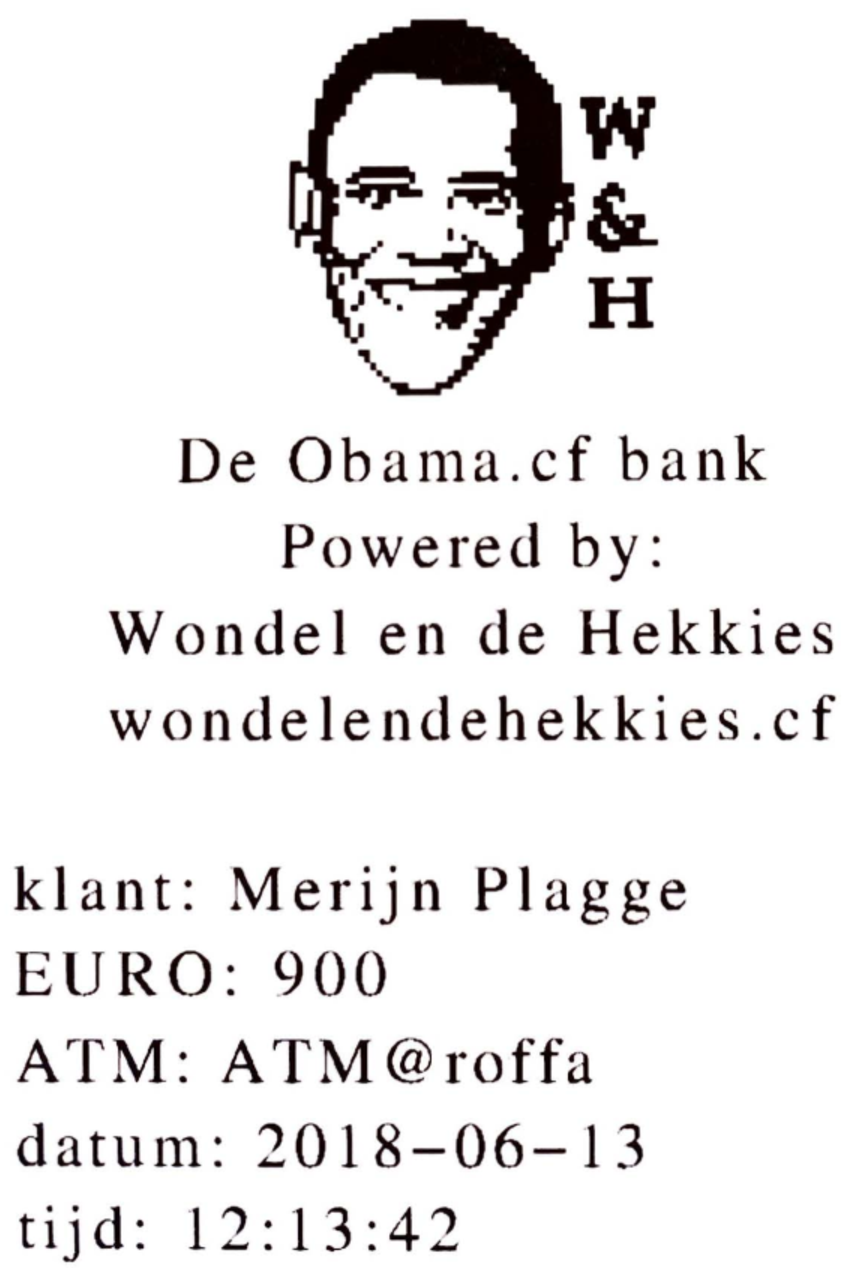
\includegraphics[height=2.0in]{obama_bon.pdf}
       \caption{Bon ontwerp}
       \label{fig: Bon ontwerp}
\end{figure}

Voor het uitgeven van bonnen hebben wij een labelprinter gebruikt.
In figuur \ref{fig: Bon ontwerp} is de bon te zien die de printer uitprint.
Hieronder is een link naar de sourcecode.

\vspace{1mm}\

\Mundus~\href{https://github.com/Gewad/Project4Bankalicious/tree/master/bonnetjesPrinten}{Code labelprinter}

\paragraph{Pseudocode uitleg}\

\lstinputlisting{Printerclass.pseudo}

\newpage

\subsection{Materiaal}

Er zijn hier een paar opties.
We kunnen bijvoorbeeld onderdelen 3d printen, maar dat zou erg duur zijn.
Het meest voor de hand liggende materiaal is triplex hout.
Dit is een redelijk goedkoop, en makkelijk verkrijgbaar materiaal.
Wij kunnen dit in het \emph{Tesla Lab} ophalen en daar direct uitsnijden.

\newpage

\section{Ontwerp \& realisatie}

\subsection{Ontwerp proces dispensers}

\paragraph{Ontwerp}

\begin{figure}[H]
       \centering
       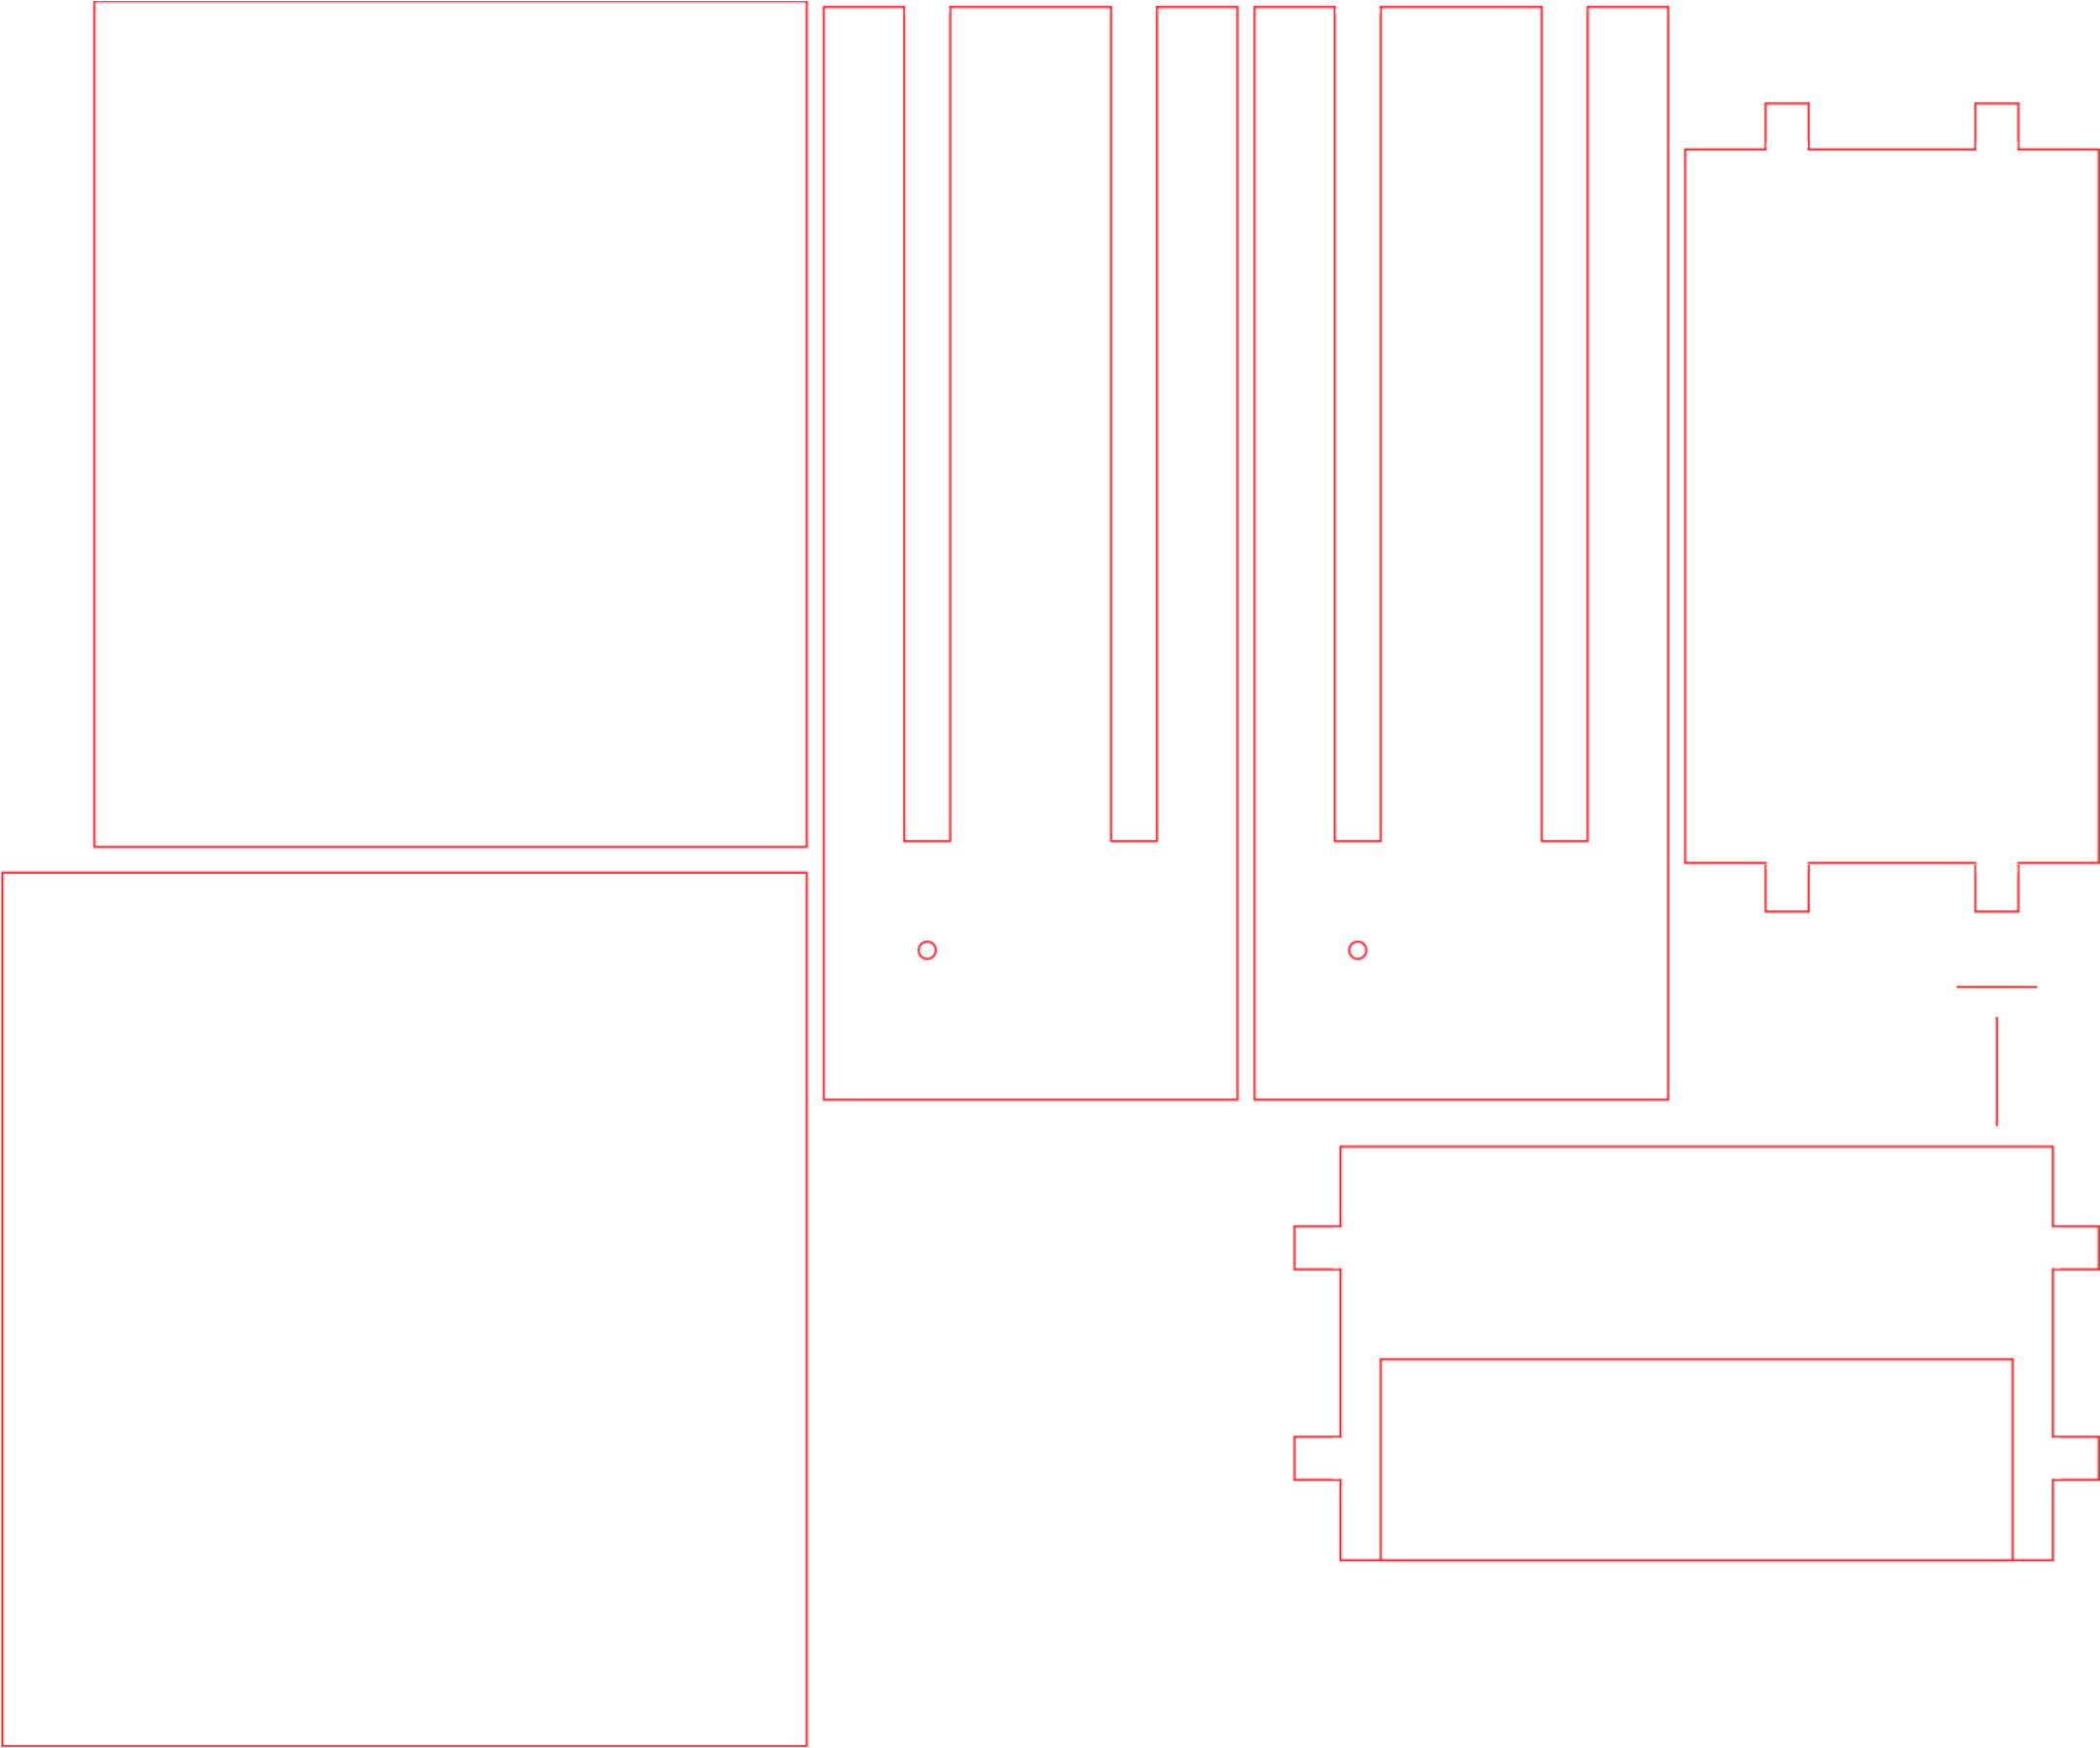
\includegraphics[height=2.0in]{dispenser.pdf}
       \caption{Dispenser ontwerp}
       \label{fig: Dispenser ontwerp}
\end{figure}

De automaat moest vier dispensers hebben.
Wij zijn begonnen met een prototype te maken voor een van deze dispensers.
In figuur \ref{fig: Dispenser ontwerp} is een bouwtekening te zien die wij hebben uitgesneden en daarna in elkaar gezet.

Tijdens het vormgeven bleek dat elastiekjes het makkelijkste werkten om het plateau waar het geld in ligt naar boven te trekken.
Ook bleek dat de as van de motor het best van lego gemaakt kon worden.
Hiervoor was het idee om de as van karton te maken, maar dit bleek niet sterk genoeg te zijn en moeilijk te maken.
Na het testen met de elastiekjes en de as hebben wij de meeste onderdelen aan elkaar gelijmd.

\paragraph{Ontwerp 2.0}

Hierna hebben we op de millimeters nauwkeurig gekeken wat de beste afstanden zouden zijn voor de uitgaven van de kaarten.
Aan de hand hiervan hebben wij een nieuwe print gemaakt en opnieuw alles getest.
Deze nieuwe print wijkt enkele millimeters af van het eerste ontwerp
Deze bleek goed, en wij hebben \emph{Ontwerp 2.0} dus uiteindelijk drie keer extra geprint.

\subsection{Bouwtekening ATM}

\begin{figure}[H]
\centering
\begin{minipage}{.5\textwidth}
  \centering
  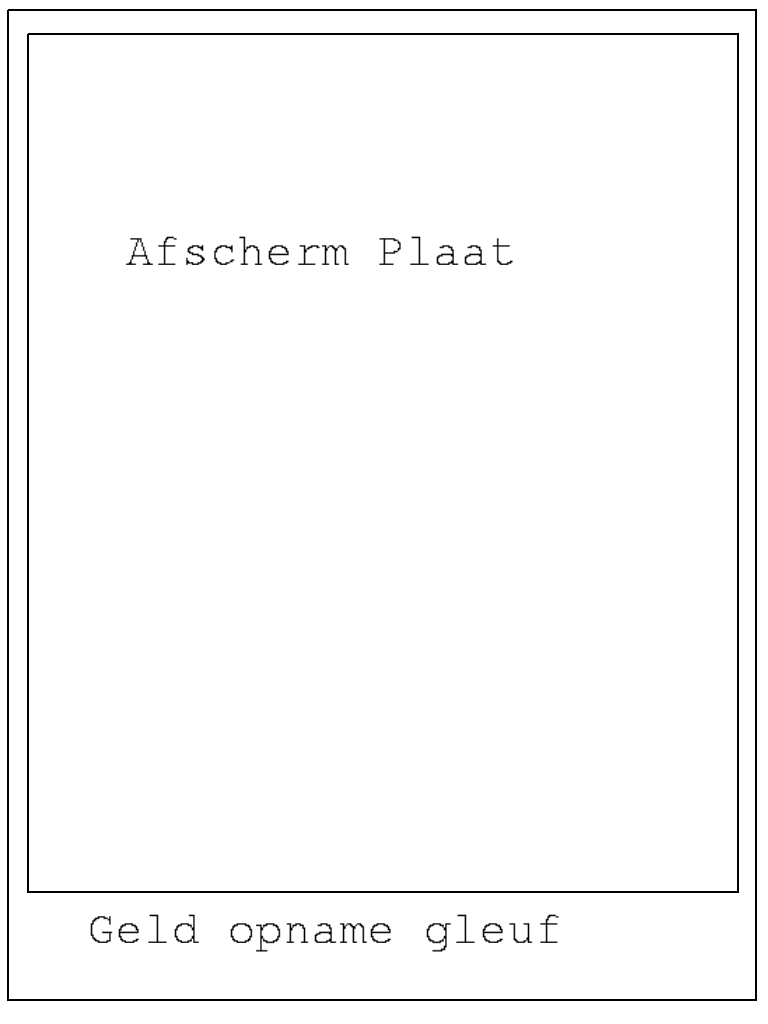
\includegraphics[height=2.5in]{voorkant.png}
  \captionof{figure}{Vooraanzicht ATM}
  \label{fig:voorkant}
\end{minipage}%
\begin{minipage}{.5\textwidth}
  \centering
  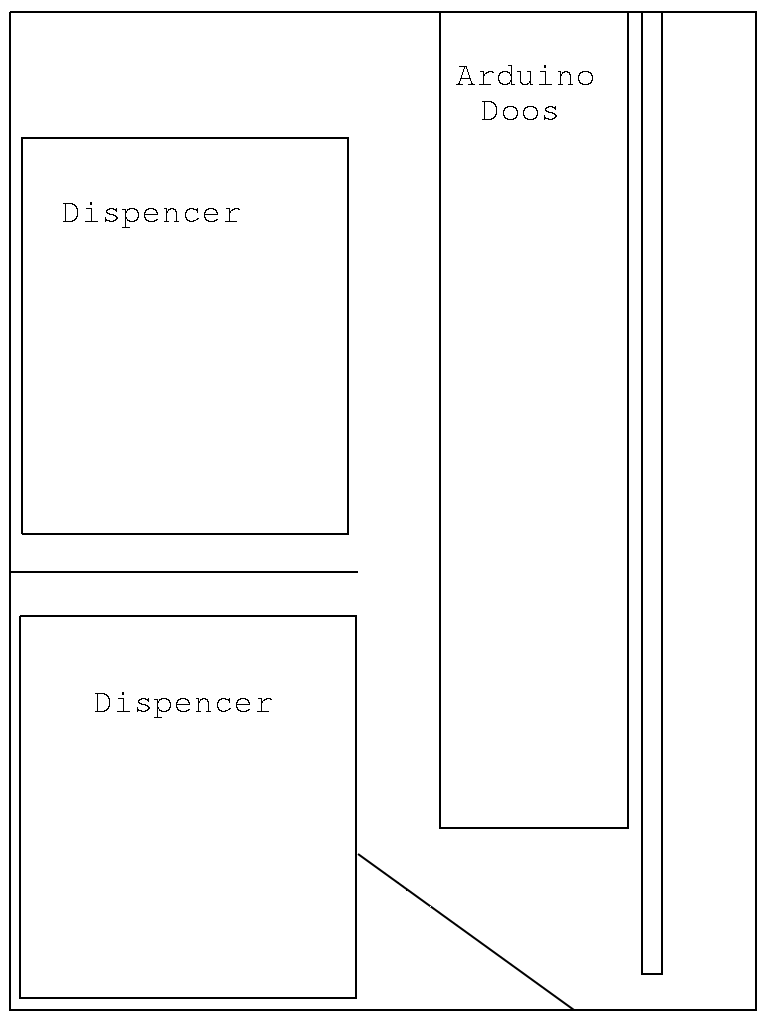
\includegraphics[height=2.5in]{zijkant.png}
  \captionof{figure}{Zijaanzicht ATM}
  \label{fig:zijkant}
\end{minipage}
\end{figure}

\begin{figure}[H]
       \centering
       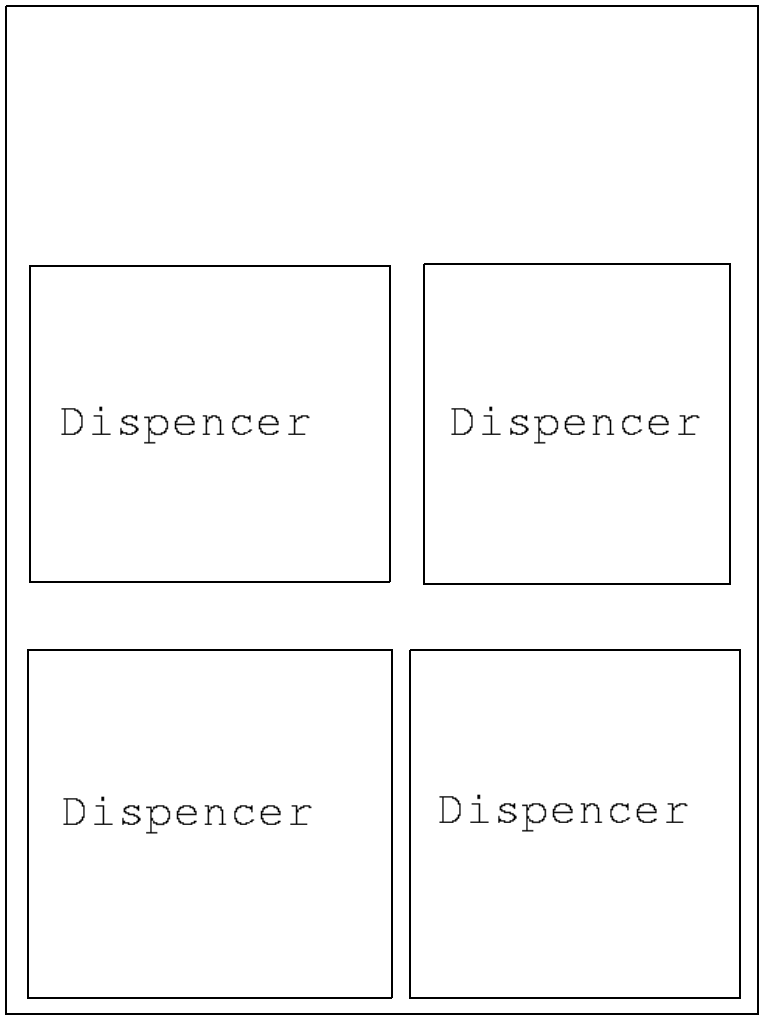
\includegraphics[height=2.5in]{achterkant.png}
       \caption{Achterkant ATM}
       \label{fig: Achteraanzicht ATM}
\end{figure}

\subsection{Electrisch schema}
\begin{figure}[H]
       \centering
       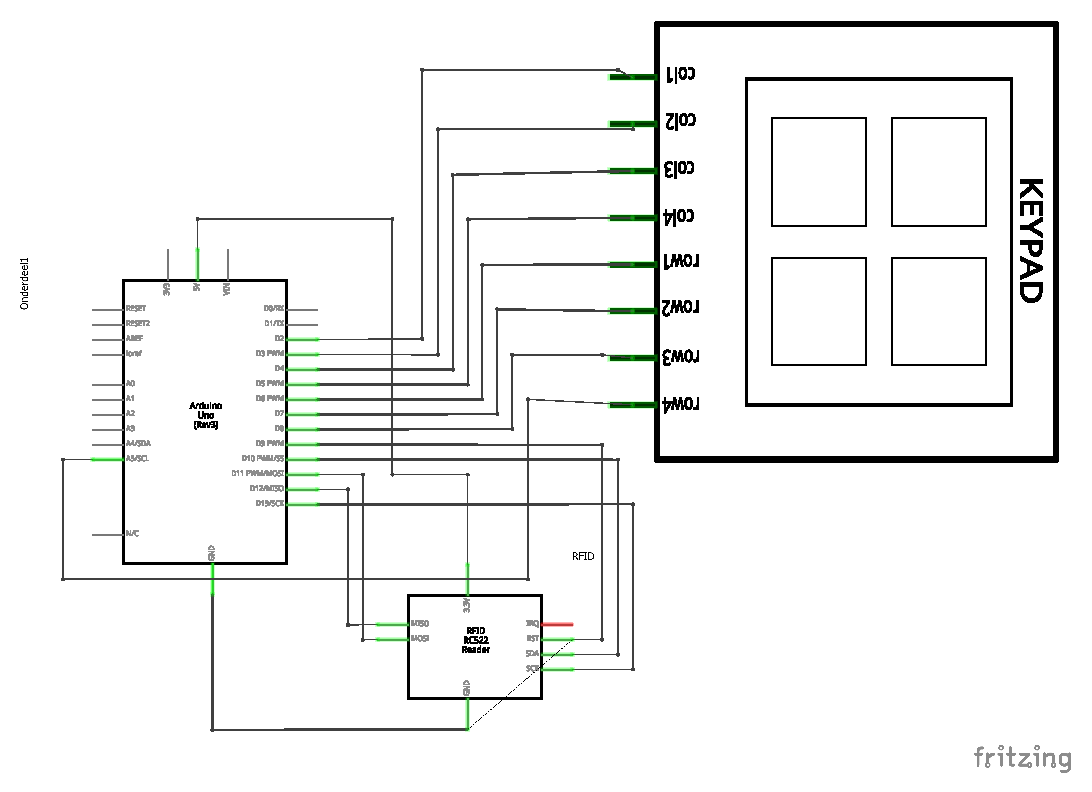
\includegraphics[height=4.5in]{Input_schema.pdf}
       \caption{Keypad en RFID}
       \label{fig: Keypad en RFID}
\end{figure}

\begin{figure}[H]
	\centering
	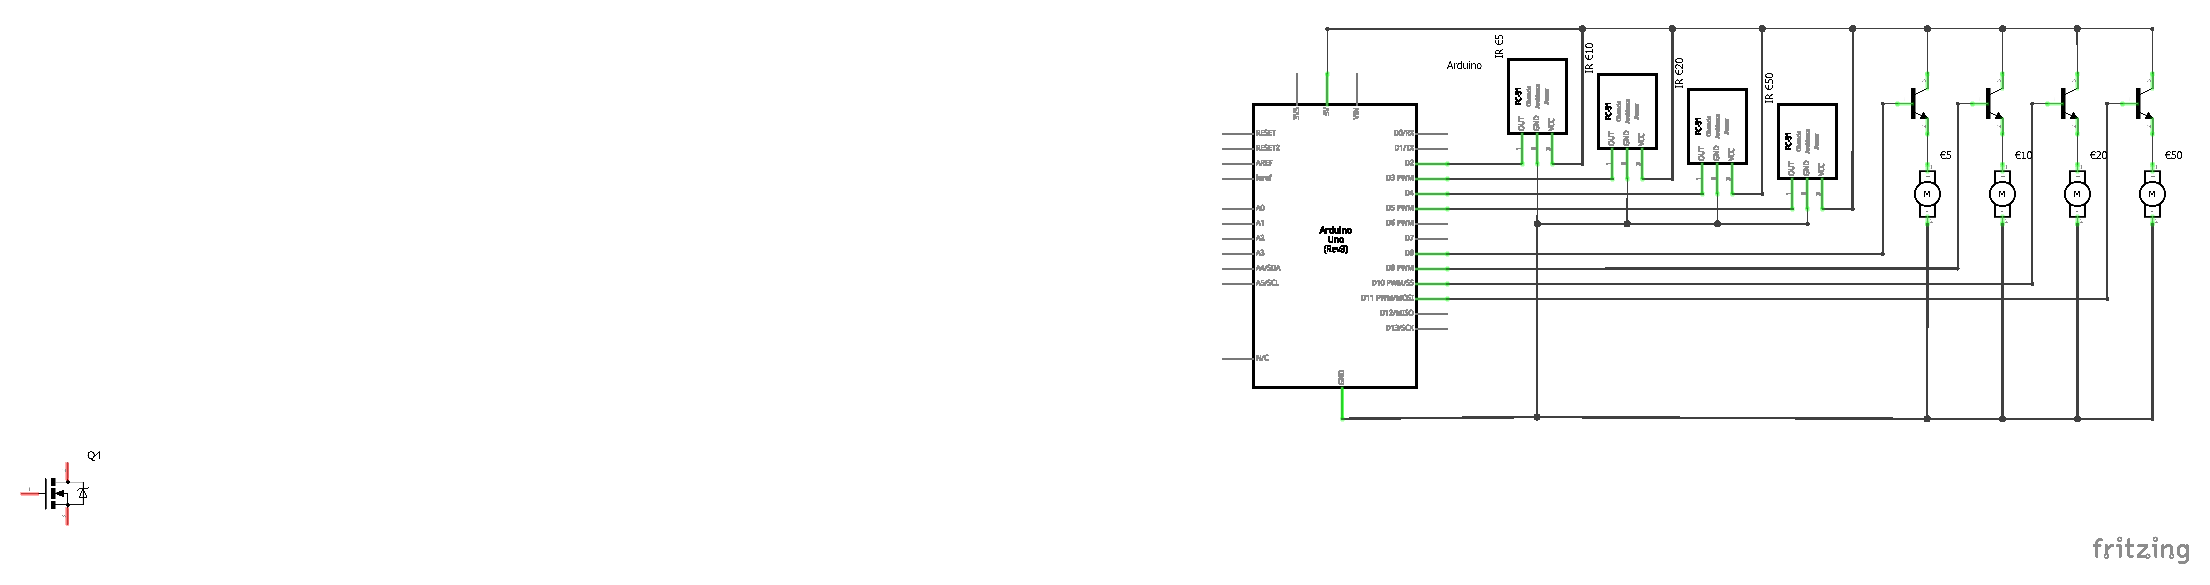
\includegraphics[height=3.0in]{Dispenser_schema.pdf}
	\caption{Dispencer Schema}
	\label{fig: Dispencer Schema}
\end{figure}

\subsection{Toepassen kwaliteitseisen}

%Boas TODO zijn wel of niet toegepast.

\subsection{Testen}

%\textbf{Aron moet dit doen}
%Tijdens het testen...
%Dit dat blijkt kut...
%Dit dat zo gefixed...

\newpage
\section{Bijlagen}

\begin{figure}[H]
       \centering
       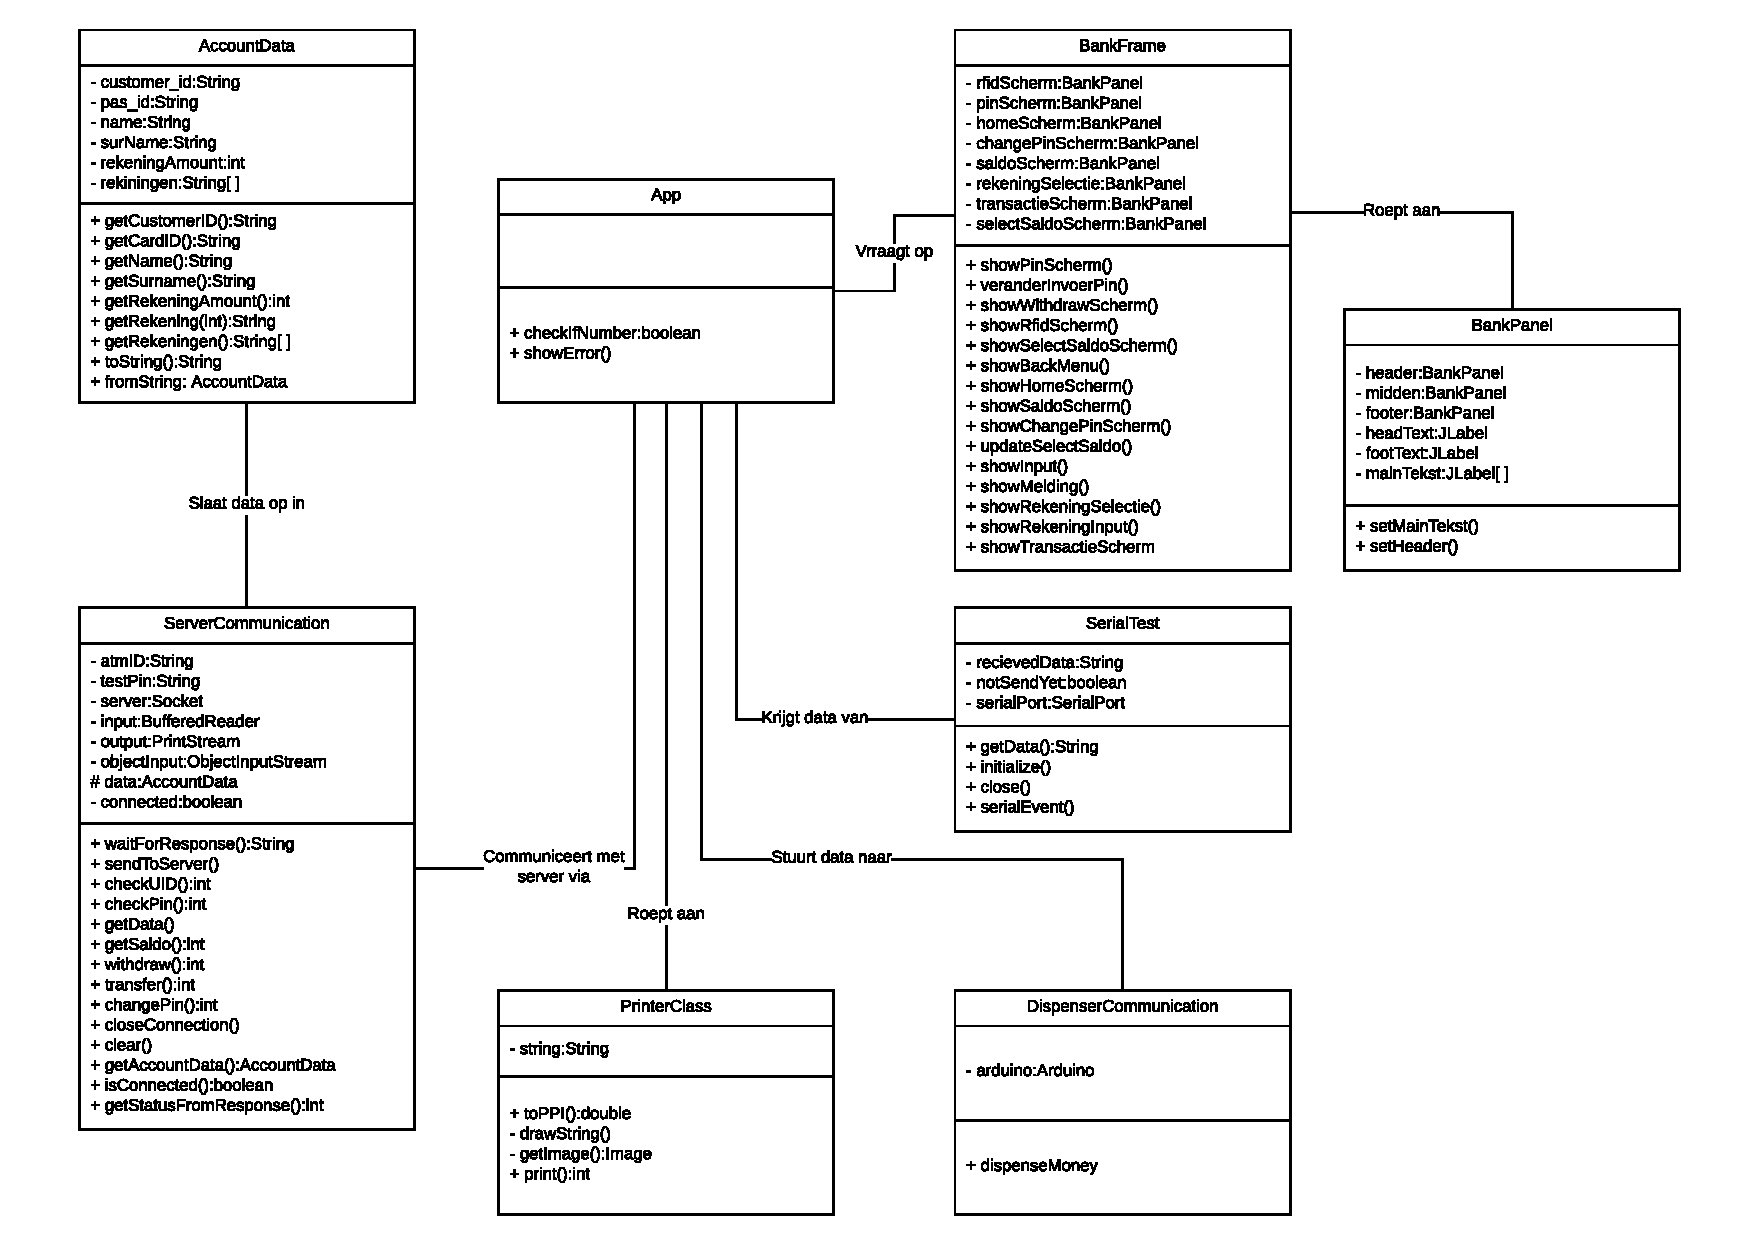
\includegraphics[height=4.5in]{Klassediagram.pdf}
       \caption{Klassediagram GUI}
       \label{fig: Klassediagram GUI}
\end{figure}

\end{document}
